\documentclass[10pt]{article}
\usepackage{mathpaper}
\begin{document}
\papertitle{第二十一章~~~一元二次方程}
\paperinformation{时间:2小时~~~~满分:120分}
\begin{questions}{\selectingintroduction}
    \question 关于$x$的一元二次方程$bx^{2} + 18x - 4c = 4$的一次项和常数项系数分别为(~~~~~~~)。
    \onp{$18$,$-4c$}{$b$,$4c+4$}{$18$,$-4c-4$}{$18$,$-4c$}
    \question 下列关于$x$的方程中,是一元二次方程的是(~~~~~~~)。
    \twp{$4x^{2} + x = (2x + 1)^{2}$}{$\frac{x^{3} + 5x^{2} + 18x}{5x} = 0$}{$( x^{2} + x )^{0} - 1 = 0$}{$- x^2 + 3 = 1$}
    \question 已知关于$x$的一元二次方程$- x^{2} + 2ax = 3b$,则(~~~~~~~)。
    \twp{$x_{1} + x_{2} = - 2a$}{$x_{1}x_{2} = 3b$}{$x_{1} - x_{2} = 2\sqrt{a^{2} - 3b}$}{$x_{1} + 2x_{2} = 2a + b$}
    \question 若关于$x$的方程$ax^{2} + bx + c = 0$有解,则下列说法正确的是(~~~~~~~)。
    \twp{方程有两个实数根}{$c = 0$时,$x$必有一解为$0$}{当$a > 0$时,方程有两个相等实数根}{$b$不可能为$0$}
    \question 若关于$x$的一元二次方程有两个解$x_{1} = 1$,$x_{2} = 2$,则这个方程可能是(~~~~~~~)。
    \twp{$x^{2} + 3x = 2$}{$x^{2} - 3x + 2 = 0$}{$x^{2} - 2x + 3 = 0$}{$x^{2} + 3x = - 2$}
    \question 如图,在平行四边形$ACBD$中,$AD=6$,$BD=\sqrt{205}$,连对角线$AB$,有$AB \bot CB$,延长$CB$至$F$,使$CB=FB$,在线段$AB$上取点$E$,连$EF$,使$EF=2AE$,则$BE$的长度为(~~~~~~~)。
    \onp{$5$}{$8$}{$10$}{$6$}
    \question 已知理想情况下物体在做自由落体运动时,下落距离$s$与时间$t$满足以下关系:$s = 4.9t^{2}$,若一个物体下落了$181.8$m,则下列等式正确的是(~~~~~~~)。
    \twp{$4.9s = {181.8}^{2}$}{$4.9t^{2} = \frac{181.8}{4.9}$}{$t = \sqrt{\frac{181.8}{4.9}}$}{$\sqrt{181.8} = t + 4.9$}
    \question 如图,为一种轻质的老式秤。某次称量时,称量的物品和秤盘的总质量为$800$g,秤砣到手拉环的距离为$s$cm时,刚好平衡。若秤盘到手拉环的距离为$5$cm,秤砣质量为$m$g,且$m$和$s$满足$m=8s+40$,则$s$的值为(~~~~~~~)。
    \onp{$30$}{$25$}{$20$}{$55$}
    \question 计算$(\frac{1+\sqrt{5}}{2})^8+(\frac{1-\sqrt{5}}{2})^8$的值为(~~~~~~~)。
    \onp{$5$}{$47$}{$34$}{$58$}
    \question 已知在$\Delta ABC$中,点$E$、$F$分别在线段$AB$、$AC$上,若$AB = AC$、$AE = EF = FC = CB$,则$\angle A$的大小为(~~~~~~~)。
    \onp{$15^{\circ}$}{$20^{\circ}$}{$22.5^{\circ}$}{$30^{\circ}$}
    \begin{figure}[!ht]
        \centering
        \subfigure[(第6题)]{
            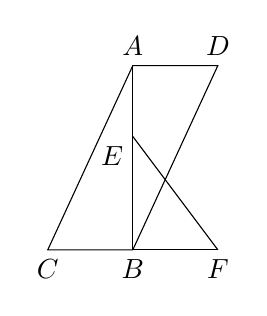
\begin{tikzpicture}[scale=0.18]
                \node[above] at (0,13) {$A$};
                \node[below] at (0,0) {$B$};
                \node[below] at (-6,0) {$C$};
                \node[below] at (6,0) {$F$};
                \node[above] at (6,13) {$D$};
                \node[below left] at (0,8) {$E$};
                \draw (-6,0)--(0,13)--(6,13)--(0,0)--cycle;
                \draw (0,13)--(0,0);
                \draw (0,0)--(6,0);
                \draw (0,8)--(6,0);
            \end{tikzpicture}
        }
        \qquad\qquad\qquad
        \subfigure[(第8题)]{
            \smallpicture{./images/T8.png}{1}
        }
        \qquad\qquad\qquad
        \subfigure[(第10题)]{
            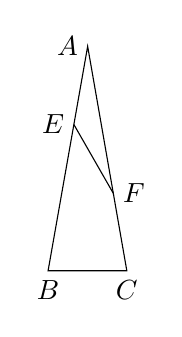
\begin{tikzpicture}[scale=0.25]
                \node[left] at (2.01,11.40) {$A$};
                \node[below] at (0,0) {$B$};
                \node[below] at (4,0) {$C$};
                \node[left] at (1.31,7.43) {$E$};
                \node[right] at (3.31,3.94) {$F$};
                \draw (2.01,11.40)--(0,0)--(4,0)--cycle;
                \draw (1.31,7.43)--(3.31,3.94);
            \end{tikzpicture}
        }
    \end{figure}
\end{questions}

\begin{questions}{\complitingintroduction}
    \question 在一元二次方程$ax^{2} + 2ax + b = 0$中,一次项系数为\complitingline{},常数项系数为\complitingline{},两根之和为\complitingline{}。
    \question 已知一元二次方程中$x^{2} - ( m^{2} - 3 )x + m = 0$,有$x_{1} + x_{2} = 2$,则$m =$\complitingline{}。
    \question 若方程$x^{2} + 2x - 3 = 0$与$x^{2} + bx + 3 = 0$有一个公共解,则$b =$\complitingline{}。
    \question 已知两实数$m$、$n$满足$m^2-3m+1=0$,$n^2-3n+1=0$,且$m \neq n$,则代数式$\sqrt{\frac{m}{n}}+\sqrt{\frac{n}{m}}$的值为\complitingline{}。
    \question 已知两实数$m$、$n$满足$m^2+3m-9=0$,$9n^2-3n-1=0$,且$mn \neq 1$,则$\frac{mn+n+mn^{2}}{n^{2}}$的值为\complitingline{}。
    \question 已知$a$、$b$、$c$为两两不相等的实数,且满足$2023(a-b)+\sqrt{2023}(b-c)+(c-a)=0$,则代数式$\frac{(b-c)(c-a)}{(a-b)^2}$的值为\complitingline{}。
\end{questions}

\begin{questions}{\answeringintroduction}
    \question 用因式分解法解下列方程。
    \begin{subquestions}
        \subquestion $x^2-6x+8=0$
        \subquestion $(2x+3)^2=x^2$
        \subquestion $x^2-2ax-5x+a^2+5a+6=0$
        \subquestion $ax^2-3a^2x-x+3a=0 \ \ \ \ \ (a \neq 0)$
    \end{subquestions}
    \addspace{}
    \question 阅读材料,完成任务。\par
    ~~~~~~~我们已经知道,对于关于$x$的一元二次方程$ax^2+bx+c=0$,由韦达定理,$x_1+x_2=-\frac{b}{a}$,$x_1x_2=\frac{c}{a}$。如果用$a$、$x_1$、$x_2$来表示$b$、$c$,那么代数式$ax^2+bx+c$可以化为$ax^2-a(x_1+x_2)x+ax_1x_2$,即$a(x-x_1)(x-x_2)$,这意味着,\textdot{对于任意的二次三项式$ax^2+bx+c$,如果一元二次方程$ax^2+bx+c=0$有实根为$x_1$,$x_2$,那么原式可因式分解为$a(x-x_1)(x-x_2)$},利用这种方法,我们可以实现二次三项式在实数范围内的因式分解。
    \begin{subquestions}
        \subquestion 在实数范围内因式分解下面的代数式,并直接写出结果:
        \begin{subsubquestions}
            \subsubquestion $x^2-x-1$
            \subsubquestion $2x^2-8x+5$
            \subsubquestion $x^4-4x^3+2x^2-4x+1$
        \end{subsubquestions}
        \subquestion 试说明为什么二次三项式$x^2+x+1$无法在实数范围内被因式分解。
    \end{subquestions}
    \newpage
    \question 已知两个一元二次方程$M:ax^{2} + bx + c = 0$和$N:cy^{2} + by + a = 0$均有两个实数根。其中$ac \neq 0$且$a \neq c$。
    \begin{subquestions}
        \subquestion 求证:如果$M$的两个实数根相等,那么$N$的两个实数根也相等。
        \subquestion 求证:如果$M$的两根符号相同,那么$N$的两根符号也相同。
    \end{subquestions}
    \addspace{}
    \question 在实数范围内解方程组$\left\{ \begin{matrix}
        (x + 1)(y + 1) = 18 \\
        x^{2}y + xy^{2} = 66 \\
        \end{matrix} \right.$。
    \addspace{}
    \question ``读书可以让人保持思想活力,让人得到智慧启发,让人滋养浩然之气''。某校为响应我市全民阅读活动,利用节假日面向社会开放学校图书馆。据统计,第一个月进馆$128$人次,进馆人次逐月增加,到第三个月末累计进馆$608$人次。
    \begin{subquestions}
        \subquestion 若进馆人次的月平均增长率相同,求进馆人次的月平均增长率。
        \subquestion 现图书馆举行活动,给每人发送活动邀请,每人转发$n$位好友即可获得书签一个,若第一轮只有一人转发,每人最多累计参与一轮转发,并恰好转发给了$n$个没有获得邀请的好友,且三轮发送后累计$13$人收到邀请,求$n$的值。
    \end{subquestions}
    \addspace{}
    \question 如图,在$\Delta ABC$中,$\angle B=90^{\circ}$,$AB=5$cm,$BC=7$cm,点$P$从点$A$开始沿$AB$边向点$B$以$1\ $cm/s的速度移动,点$Q$从点$B$开始沿$BC$边向点$C$以$2\ $cm/s的速度移动,若$P$、$Q$同时出发,且一点到达目标点,两点均立刻停止运动,则:
    \begin{subquestions}
        \subquestion 在几秒后,$S_{\Delta PBQ}=4\ $cm$^2$?
        \subquestion 在几秒后,$PQ=5\ $cm?
    \end{subquestions}
    \begin{figure}[!h]
        \raggedleft
        \subfigure[(第22题)]{
    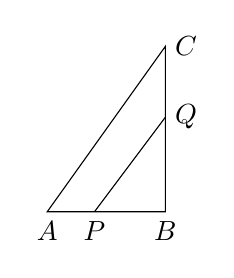
\begin{tikzpicture}[scale=0.3]
        \node[below] at (-5,0) {$A$};
        \node[below] at (0,0) {$B$};
        \node[right] at (0,7) {$C$};
        \node[below] at (-3,0) {$P$};
        \node[right] at (0,4) {$Q$};
        \draw (-5,0)--(0,0)--(0,7)--cycle;
        \draw (-3,0)--(0,4);
    \end{tikzpicture}}
    \end{figure}
    \newpage
    \question
    \begin{subquestions}
        \subquestion 已知$x$为实数,求代数式$x^2-8x+5$的最小值。
        \subquestion 已知$x$为实数,求代数式$\frac{x^2+x+1}{x^2+1}$的取值范围。
        \subquestion 已知$x$、$y$均为实数,直接写出代数式$-3x^2+3xy+6x-y^2$的最大值。
    \end{subquestions}
    \addspace{}
    \question 如图,在平面直角坐标系中,$A$在$y$轴正半轴上,$B$、$C$为$x$轴上两动点。
    \begin{subquestions}
        \subquestion 如图1,$A(0,4)$,$B$从$(-5,0)$出发,$C$从$(5,0)$出发,都以每秒$t$个单位长度向$x$轴负半轴方向运动,连$AB$、$AC$。
        \begin{subsubquestions}
            \subsubquestion 当$\angle BAC=90^{\circ}$时,直接写出直线$AC$的解析式。
            \subsubquestion 在\circnum{1}的条件下,若$P$为线段$AC$上一点,作$PM$垂直于$x$轴于点$M$,作$PN$垂直于$y$轴于点$N$,求四边形$OMPN$面积的最大值。
        \end{subsubquestions}
        \subquestion 如图2,直线$AB:y=-\sqrt{3}x+b$,$C$在$B$左侧,$E(m,n)$为射线$AB$上一点,$CD=2m$,连接$AC$,$CE$,$DE$,若$AC=6$,$DE=5$,求$CE$的取值范围。
    \end{subquestions}
    \begin{figure}[htb]
        \centering
        \subfigure[(1)]{
        \begin{tikzpicture}[>=Stealth,scale=0.65]
            \draw[->] (-6.5,0)--(6.5,0) node[below] {$x$};
            \draw[->] (0,-1)--(0,6.5) node[left] {$y$};
            \node[below right] at (0,0) {$O$};
            \node[above right] at (0,4) {$A$};
            \node[below] at (-5,0) {$B$};
            \node[below] at (5,0) {$C$};
            \draw (-5,0)--(0,4)--(5,0);
        \end{tikzpicture}
        }
        \qquad
        \subfigure[(2)]{
        \begin{tikzpicture}[>=Stealth,scale=0.65]
            \draw[->] (-4.5,0)--(4,0) node[below] {$x$};
            \draw[->] (0,-1)--(0,6.5) node[left] {$y$};
            \node[below right] at (0,0) {$O$};
            \node[left] at (0,5) {$A$};
            \node[right] at (0.5,4.13397) {$E$};
            \node[below] at (-0.4,0) {$C$};
            \node[below right] at (0.6,0) {$D$};
            \node[below] at (2.88675,0) {$B$};
            \draw (0,5)--(2.88675,0);
            \draw (0,5)--(-0.4,0);
            \draw (-0.4,0)--(0.5,4.13397);
            \draw (0.6,0)--(0.5,4.13397);
        \end{tikzpicture}}
        \caption*{(第24题)}
    \end{figure}
\end{questions}
\end{document}